\documentclass[a4paper,14pt]{article}
\usepackage[utf8]{inputenc}
\usepackage{mathtext}
\usepackage[T2A]{fontenc}
\usepackage[margin=1in]{geometry}
\usepackage{booktabs}
\usepackage{graphicx, wrapfig}
\usepackage[english,russian]{babel}	% локализация и переносы
\usepackage{tabularx}
\usepackage{amsmath,amsfonts,amssymb,amsthm,mathtools}
\usepackage{tikz,graphics,color,fullpage,float,epsf,caption,subcaption}
\usepackage{etoolbox} 
\usepackage{enumitem}
\usepackage{siunitx}
\usepackage{textcomp}

\newcommand*{\hm}[1]{#1\nobreak\discretionary{}
{\hbox{$\mathsurround=0pt #1$}}{}}

\usepackage{extsizes}

\usepackage{geometry} 
	\geometry{top=30mm}
	\geometry{bottom=40mm}
	\geometry{left=30mm}
	\geometry{right=20mm}

\usepackage{setspace}
\onehalfspacing

\usepackage{soulutf8} 


\setlength{\parskip}{1em}
\setlength{\parindent}{0em}
\begin{document}
\begin{titlepage}
    \pagestyle{empty}
\end{titlepage}
\linespread{1}

\thispagestyle{empty} 
\begin{center}
	\textit{Федеральное государственное автономное образовательное учреждение высшего образования }
	\vspace{0.5ex}
	
	\textbf{<<МОСКОВСКИЙ ФИЗИКО-ТЕХНИЧЕСКИЙ ИНСТИТУТ>>}
\end{center}
\vspace{13ex}
\begin{flushright}
	\noindent
	\textit{Манро Эйден Форбс}
	\\
	\textit{студент 2 курса группы Б01-307}
\end{flushright}
\begin{center}
	\vspace{13ex}
	\so{\textbf{ВОПРОС ПО ВЫБОРУ}}
	\vspace{1ex}
	
	по курсу общей физики <<Оптика>>
	
	на тему:
	
	\textbf{Зоны Шустера и спираль Корню}
	
	\vfill
	Москва 2025
\end{center}

\newpage

\section{Введение}
В одномерных задачах, например при рассмотрении дифракции на прямоугольной щели, разбиение волнового фронта на кольцевые зоны нецелесообразно. Лучше разбивать волновой фронт на полосатые зоны, называемые зонами Шустера (1851-1934).

\section{Теория}

\begin{wrapfigure}{l}{0.6\textwidth}
    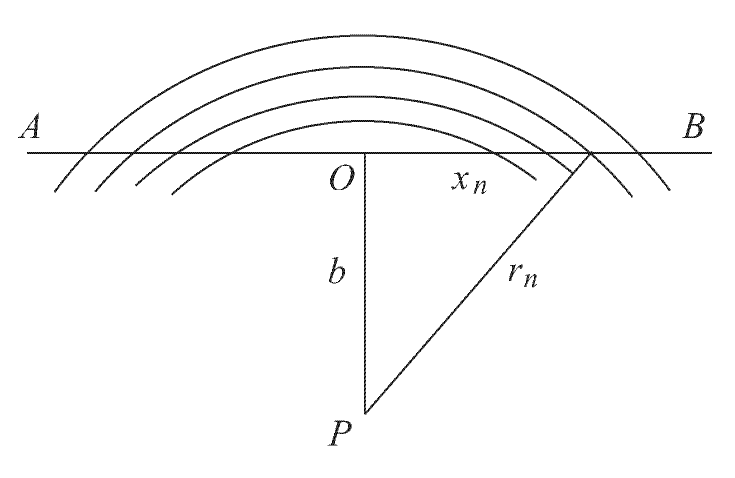
\includegraphics[width = 0.6\textwidth]{govno.png}
    \caption{}\label{wrap-fig:govno}
\end{wrapfigure}

Ограничимся случаем когда волновой фронт плоский, хотя обобщение на случай сферического фронта и не встречает никаких препятствий. Пусть плоскость волнового фронта АВ перпендикулярна к плоскости рис. \ref{wrap-fig:govno}. Обозначим через $b$ длину перпендикуляра $РО$, опущенного из точки наблюдения на волновой фронт. Проведем цилиндрические коаксиальные поверхности, ось которых проходит через точку Р перпендикулярно к плоскости рисунка, а радиусы равны $b$, $b+\lambda/2$, $b+2(\lambda/2)$, ...
Тогда волновой фронт разобьется на прямоугольные полосы, которые и называются зонами Шустера. Центральную зону условимся считать за две зоны: одна расположена справа, а другая слева от точки $О$. 
Тогда \( r_n^2 = b^2 + x_n^2 \), \( r_{n-1}^2 = b^2 + x_{n-1}^2 \), а потому
\[
r_n^2 - r_{n-1}^2 = x_n^2 - x_{n-1}^2.
\]
Приближённо
\[
r_n^2 - r_{n-1}^2 = (r_n + r_{n-1})(r_n - r_{n-1}) = 2b(\lambda/2) = b\lambda.
\]

Таким образом, получаем рекуррентное соотношение
\[
x_n^2 - x_{n-1}^2 = b\lambda,
\]
из которого могут быть найдены все \( x_n \). Так как \( x_0 = 0 \), то
\[
x_1 = \sqrt{b\lambda}, \quad x_2 = \sqrt{2b\lambda}, \quad \dots, \quad x_n = \sqrt{nb\lambda}.
\]

Ширины последовательных зон Шустера будут
\[
\sqrt{b\lambda}, \quad (\sqrt{2} - 1)\sqrt{b\lambda}, \quad (\sqrt{3} - \sqrt{2})\sqrt{b\lambda}, \dots.
\]

Они монотонно убывают и в пределе, когда \( r \to \infty \), стремятся к \(\lambda/2\), как это ясно из их построения. (Впрочем высшие зоны не играют роли. Имеют значение не только несколько десятков первых зон Шустера).

Как и в случае зон Френеля, применим теперь графический метод. Каждую зону Шустера разобьем на узкие полоски и будем изображать колебание в точке Р, вносимое отдельной полоской, вектором на векторной диаграмме. Затем перейдем к пределу, устремляя к нулю ширину каждой полоски. В результате чего получится плавная кривая, называемая спиралью Корню (1841-1902). Она состоит из двух симметричных ветвей, бесконечное число раз обвивающихся вокруг <<фокусов>> $F$ и $F'$ и неограниченно приближающихся к ним. 

\begin{figure}[h]
    \centering
    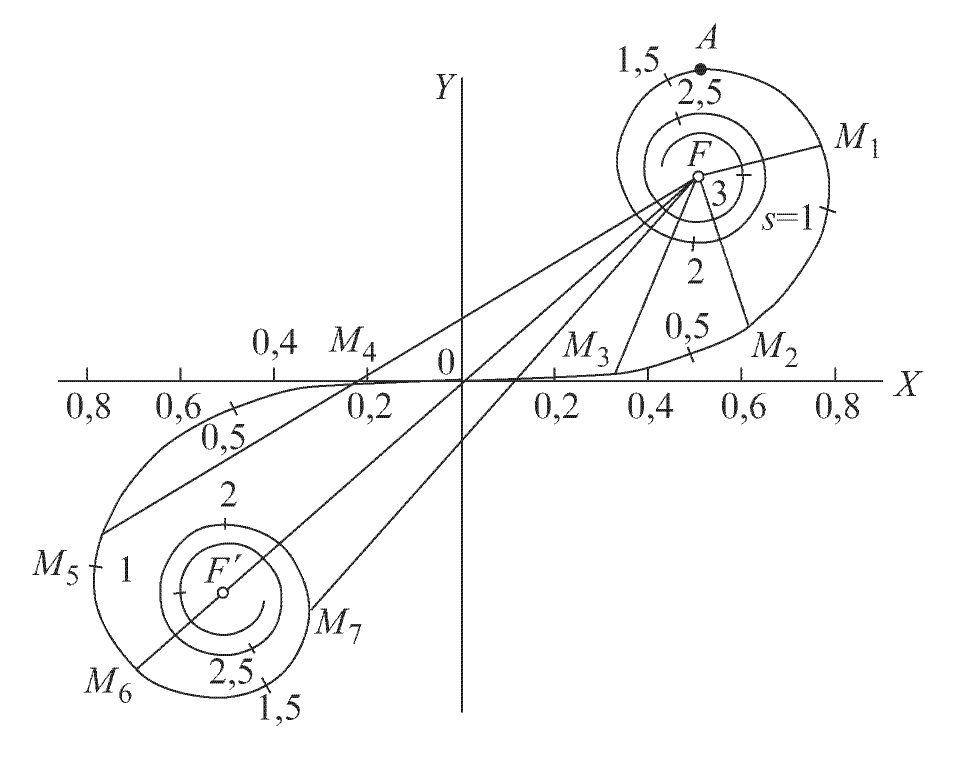
\includegraphics[width = 0.8\textwidth]{korny.png}
    \caption{}\label{fig:spiral_korny}
\end{figure}

Верхняя ветвь представляет действие правой половины волнового фронта, нижняя — левой. Отличие каждой из ветвей от соответствующей спирали Френеля обусловлено более быстрым убыванием начальных зон Шустера, чем зон Френеля. Колебание, возбуждаемое первой правой зоной Шустера, изображается вектором \( \overrightarrow{OA} \), второй правой — вектором \( \overrightarrow{AB} \), двумя первыми правыми зонами вместе — вектором \( \overrightarrow{OB} \) и т.д. (все эти векторы на рис. \ref{fig:spiral_korny} не проведены). Колебание, возбуждаемое всем волновым фронтом, представляется вектором \( \overrightarrow{F'F} \), соединяющим фокусы спирали Корню. По мере приближения к фокусам амплитуды колебаний становятся все меньше и меньше и в пределе обращаются в нуль.


При нахождении уравнения спирали Корню надо учесть, что реально всегда приходится иметь дело не с бесконечными, а с ограниченными волновыми фронтами, причём заметная интенсивность наблюдается лишь при малых углах дифракции. Поэтому в формуле $E_{P} = \int \frac{1}{r r^{\prime}} e^{i \Phi(\mathbf{R})} \, dF$ изменения знаменателей \( r \) и \( r' \) (а также уже отброшенных ранее ослабляющих множителей \( K(\alpha) \)) можно не принимать во внимание. Если нас интересует только относительное распределение интенсивности, то можно положить \( rr' = 1 \). В плоскости волнового фронта фазу можно представить в виде \( \Phi = \omega t - kr \) (здесь произведено переобозначение: в формуле (41.1) расстояние \( r \) обозначалось через \( r' \)).

Примем волновой фронт за координатную плоскость \( XY \), а начало координат поместим в точке \( O \). Тогда \( r^2 = b^2 + (x^2 + y^2) \), а следовательно, 
\[
r - b = \frac{x^2 + y^2}{2b} + \ldots
\]
Члены высших степеней можно отбросить, если даже они добавляют в фазу слагаемые порядка \( \pi \) и больше. Дело в том, что такие члены, как это видно из формы спирали Корню, не меняя общего характера дифракционной картины, производят в ней только практически незаметные смещения высших дифракционных максимумов и минимумов. Кроме того, высшие дифракционные максимумы и минимумы следуют друг за другом столь часто, что для их реального осуществления требуются точечные источники света высокой степени монохроматичности. В противном случае все дифракционные полосы высших порядков размываются и переходят в равномерно освещённый фон. Отбросим все фазовые множители, не влияющие на относительное распределение интенсивности светового поля. Тогда поле в точке наблюдения \( P \) представится интегралом
\[
E_P = \iint e^{-ik(x^2 + y^2)/(2b)} \, dx \, dy.
\]

Интегрирование должно быть выполнено по всей открытой поверхности волнового фронта. Допустим, что в направлении оси \( Y \) она простирается достаточно далеко в обе стороны. Тогда интегрирование по \( y \) можно выполнить в пределах от \( -\infty \) до \( +\infty \), в результате чего появится постоянный множитель, не представляющий интереса. Интегрирование по \( x \) произведём от нуля, считая верхний предел \( x \) переменным (он может быть и положительным, и отрицательным). Вместо \( x \), как это принято, введём новую переменную \( s \) по формуле \( kx^2/b = \pi s^2 \). Тогда
\[
E_P = \int_0^s e^{-i\pi s^2/2} \, ds, \tag{1}
\]
\[
E_P^* = \int_0^s e^{i\pi s^2/2} \, ds. \tag{2}
\]

При изображении колебаний можно пользоваться как выражением (1), так и комплексно сопряжённым с ним (2). При построении спирали Корню обычно применяют выражение (2). Оно и представляет уравнение спирали Корню в комплексной форме. Если координатные оси выбраны так, как указано на рис. \ref{fig:spiral_korny}, то в прямоугольных координатах уравнение спирали Корню запишется в виде
\[
X(s) = \int_{0}^{s} \cos \frac{\pi s^2}{2} \, ds, \quad Y(s) = \int_{0}^{s} \sin \frac{\pi s^2}{2} \, ds.
\tag{3}
\]

Входящие сюда интегралы называются \textbf{интегралами Френеля}. Очевидно,
\[
X(s) = -X(-s), \quad Y(s) = -Y(-s),
\]
т.е. кривая (3) симметрична относительно начала координат.

Полагая \( s = \infty \), находим координаты фокусов спирали Корню:
\[
X_F = Y_F = \frac{1}{2}, \quad X_{F'} = Y_{F'} = -\frac{1}{2}.
\]

Впрочем, для многих целей проще пользоваться непосредственно комплексной формой (2). В частности, для дифференциала дуги спирали Корню из (2) находим: \( \left|e^{i\pi s^2/2} \, ds\right| = |ds| \). Отсюда следует, что параметр \( s \) есть длина дуги спирали, отсчитываемая от начала координат \( O \).

Если \( \tau \) — угол между касательной к спирали Корню и осью \( X \), то \( \tan \tau = \frac{dY}{dX} = \tan \left(\frac{\pi s^2}{2}\right) \), а потому
\[
\tau = \frac{\pi s^2}{2}.
\tag{4}
\]

При \( s = 0 \) угол \( \tau = 0 \), т.е. в начале координат кривая касается оси \( X \). При \( s = 1 \) касательная вертикальна и идёт вверх. При \( s = \sqrt{2} \), \( \tau = \pi \) касательная снова горизонтальна, но идёт в отрицательном направлении оси \( X \). При \( s = \sqrt{3} \), \( \tau = \frac{3\pi}{2} \) она вертикальна и идёт вниз. При \( s = 2 \), \( \tau = 2\pi \) касательная принимает исходное — горизонтальное — направление. Формула (4) позволяет наглядно проследить, как кривая обвивается вокруг фокусов \( F \) и \( F' \), делая при этом бесконечное число оборотов. Эта формула особенно полезна в том отношении, что она позволяет по заданному параметру \( s \) легко находить соответствующую точку на спирали Корню.

Из формулы (4) получаем формулу для кривизны спирали Корню:
\[
\frac{1}{R} = \frac{d\tau}{ds} = \pi s.
\]

Длина всей спирали Корню бесконечна, а потому при приближении к фокусам её кривизна стремится к бесконечности.

\textbf{3.} При работе со спиралью Корню надо знать значение параметра \( s \). Его легко найти, зная на экране расстояние \( x \) точки наблюдения от центра картины \( O \) (см. рис. \ref{wrap-fig:govno}). Вычислив ширину первой зоны Шустера \( \sqrt{\lambda b} \), находим далее \( s = x\sqrt{2/(\lambda b)} \).

Рассмотрим в качестве примера дифракционную картину от прямолинейного края экрана (рис. \ref{wrap-fig:hueta}). Где бы ни находилась точка наблюдения \( P \), для неё всегда будет открыт правый край волнового фронта. На векторной диаграмме (см. рис. \ref{fig:spiral_korny}) колебание в точке наблюдения представится вектором \( M_n \dot{F} \), конечная точка которого всегда находится в верхнем фокусе \( F \), а начальная \( M_n \) лежит где-то на спирали Корню. Если, сохраняя неизменным положение конечной точки \( F \), перемещать начальную точку \( M_n \) вдоль спирали Корню (положения \( M_1, M_2, M_3, \ldots \)), то таким путём можно получить распределение амплитуд и интенсивности колебаний света по всему экрану.

\begin{wrapfigure}{l}{0.5\textwidth}
    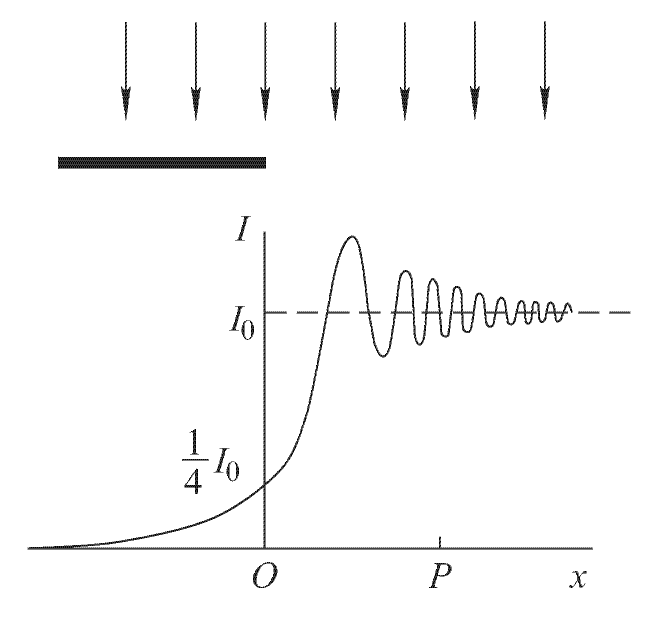
\includegraphics[width = 0.5\textwidth]{hueta.png}
    \caption{}\label{wrap-fig:hueta}
\end{wrapfigure}

Обозначим через \( a_0 = |F F'| \) и \( I_0 = a_0^2 \) амплитуду и интенсивность волны, когда открыт весь волновой фронт. Когда точка наблюдения \( P \) находится на границе геометрической тени, то колебание представится вектором \( O \dot{F} = \frac{1}{2} F' \dot{F} \). Ему соответствует амплитуда \( a_0/2 \) и интенсивность \( I_0/4 \). При перемещении точки \( P \) в освещённую область экрана изображающая точка \( M_n \) начнёт перемещаться по нижней ветви спирали Корню, а амплитуда и интенсивность колебаний будут последовательно проходить через максимумы и минимумы. Максимальная амплитуда, как видно из рис. \ref{fig:spiral_korny}, составляет \( 1,\!12a_0 \), а интенсивность \( 1,\!25I_0 \); минимальные значения их соответственно \( 0,\!89a_0 \) и \( 0,\!78I_0 \). При дальнейшем продвижении в освещённую область интенсивность асимптотически приближается к \( I_0 \). При погружении точки \( P \) в область геометрической тени изображающая точка \( M_n \) перемещается по верхней ветви спирали Корню. При этом по мере погружения в указанную область интенсивность света монотонно убывает и асимптотически стремится к нулю.

Распределение интенсивности графически представлено на рис. \ref{wrap-fig:hueta}. Таким образом, нет резкой границы между светом и тенью: в области геометрической тени интенсивность света убывает непрерывно и монотонно, а освещённая область расщепляется в дифракционные полосы. На рис. \ref{fig:168} показана дифракционная картина, наблюдаемая при дифракции света на крае экрана. Таким же путём можно рассчитать дифракционную картину на щели или длинном прямоугольном экране. На рис. \ref{fig:169} показана тень проволоки от точечного (или линейного) источника.

\begin{figure}[h]
    \centering
    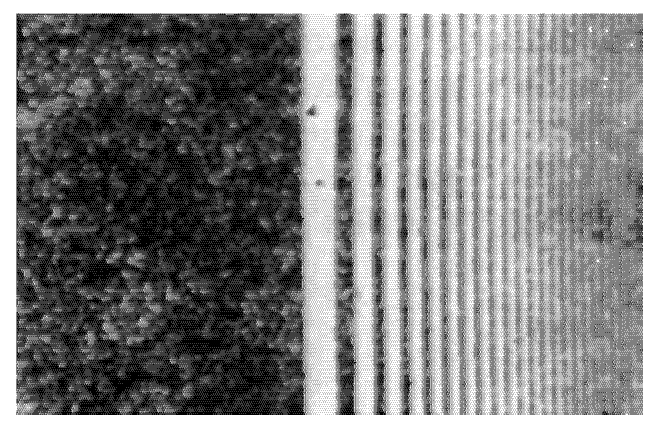
\includegraphics[width = 0.6\textwidth]{168.png}
    \caption{}\label{fig:168}
\end{figure}

\begin{figure}[h]
    \centering
    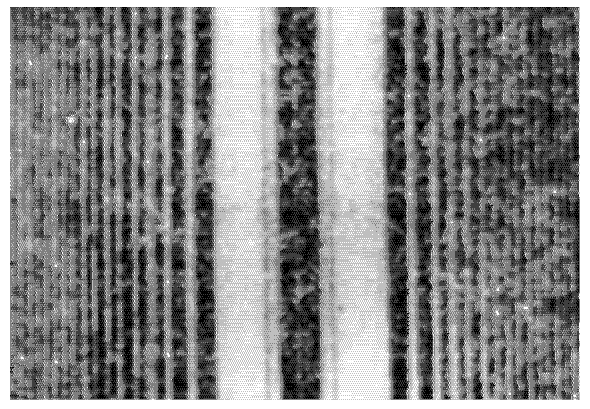
\includegraphics[width = 0.6\textwidth]{169.png}
    \caption{}\label{fig:169}
\end{figure}

\section{Литература}
$\left[1\right]$ Сивухин Д.В. Общий курс физики. Учеб. пособие: Для вузов, В 5 т. Т. \MakeUppercase{\romannumeral 4}. Оптика. - 3-е изд., стереот. - М.: ФИЗМАТЛИТ, 2005. - 792 с.

\end{document}
